% !TEX program = xelatex
% !BIB program = bibtex

\documentclass[conference]{IEEEtran}
\IEEEoverridecommandlockouts
% The preceding line is only needed to identify funding in the first footnote. If that is unneeded, please comment it out.
\usepackage{cite}
\usepackage{amsmath,amssymb,amsfonts}
\usepackage{algorithmic}
\usepackage{graphicx}
\usepackage{textcomp}
\usepackage{xcolor}
\usepackage{tikz}
\usetikzlibrary{shapes,arrows,decorations.pathmorphing,backgrounds,positioning,fit,petri,calc}
\usepackage[colorlinks,linkcolor=black,anchorcolor=black,citecolor=black, urlcolor=blue]{hyperref}
\usepackage{caption}
\usepackage{subcaption}
\usepackage{cleveref}
\captionsetup[table]{skip = 3pt}
\captionsetup[subfigure]{subrefformat=simple}
\usepackage{multirow}
\usepackage{booktabs}
\usepackage{etoolbox,siunitx}
\usepackage{array}
\newcolumntype{P}[1]{>{\centering\arraybackslash}p{#1}}

\sisetup{detect-weight,mode=text}
% for avoiding siunitx using bold extended
\renewrobustcmd{\bfseries}{\fontseries{b}\selectfont}
\renewrobustcmd{\boldmath}{}
% abbreviation
\newrobustcmd{\B}{\bfseries}

\renewcommand{\arraystretch}{1.3}

\DeclareMathOperator*{\argmin}{\arg\!\min}

\def\BibTeX{{\rm B\kern-.05em{\sc i\kern-.025em b}\kern-.08em
    T\kern-.1667em\lower.7ex\hbox{E}\kern-.125emX}}
    
\tikzset{%
  every neuron/.style={
    circle,
    draw,
    minimum size=0.5cm
  },
  neuron missing/.style={
    draw=none, 
    scale=2,
    text height=0.333cm,
    execute at begin node=$\vdots$
  },
}

\begin{document}


\title{Article Template \\
% {\footnotesize \textsuperscript{*}Note: Sub-titles are not captured in Xplore and
% should not be used}
% \thanks{Identify applicable funding agency here. If none, delete this.}
}

% 1\textsuperscript{st}

\author{\IEEEauthorblockN{Hao Wen}
\IEEEauthorblockA{\textit{Dept. Computer Science \& Technology} \\
\textit{Tsinghua University}\\
Beijing, China \\
wenh-06-10@tsinghua.edu.cn}
% \and
% \IEEEauthorblockN{Wenjian Yu}
% \IEEEauthorblockA{\textit{Dept. Computer Science \& Technology} \\
% \textit{Tsinghua University}\\
% Beijing, China \\
% yu-wj@tsinghua.edu.cn}
% \and
% \IEEEauthorblockN{Yuanqing Wu}
% \IEEEauthorblockA{\textit{JingDong Health Inc.}\\
% Beijing, China \\
% wuyuanqing@jd.com}
% \and
% \IEEEauthorblockN{Lu Wang}
% \IEEEauthorblockA{\textit{}\\
% Beijing, China \\
% @jd.com}
% \and
% \IEEEauthorblockN{Jun Zhao}
% \IEEEauthorblockA{\textit{JingDong Health Inc.}\\
% Beijing, China \\
% zhaojun10@jd.com}
% \and
% \IEEEauthorblockN{Xiaolong Liu}
% \IEEEauthorblockA{\textit{JingDong Health Inc.}\\
% Beijing, China \\
% liuxiaolong10@jd.com}
% \and
% \IEEEauthorblockN{Zhexiang Kuang}
% \IEEEauthorblockA{\textit{JingDong Health Inc.}\\
% Beijing, China \\
% kuangzhexiang@jd.com}
% \and
% \IEEEauthorblockN{Rong Fan}
% \IEEEauthorblockA{\textit{JingDong Health Inc.}\\
% Beijing, China \\
% fanrong18@jd.com}
% \and
% \IEEEauthorblockN{Shuai Yang}
% \IEEEauthorblockA{\textit{Jing Dong Health Inc.}\\
% Beijing, China \\
% yangshuai15@jd.com}
% \and
% \IEEEauthorblockN{Jeethan Jue Zhang}
% \IEEEauthorblockA{\textit{Jing Dong Health Inc.}\\
% Beijing, China \\
% zhangjue@jd.com}
% \and
% \IEEEauthorblockN{Lei Han}
% \IEEEauthorblockA{\textit{Jing Dong Health Inc.}\\
% Beijing, China \\
% hanlei70@jd.com}
}

\maketitle

\setcounter{footnote}{0}

\begin{abstract}

\end{abstract}

\begin{IEEEkeywords}

\end{IEEEkeywords}

\section{Introduction}
\label{sec:intro}

\section{Related Work}
\label{sec:related_work}

\section{Method}
\label{sec:method}

\section{Experiments and Discussion}
\label{sec:experiments}

\section{Conclusions and Future Work}
\label{sec:conclusions_fw}


\section{Code availability}





\begin{figure}
\centering
\begin{subfigure}[b]{.4\textwidth}
\centering
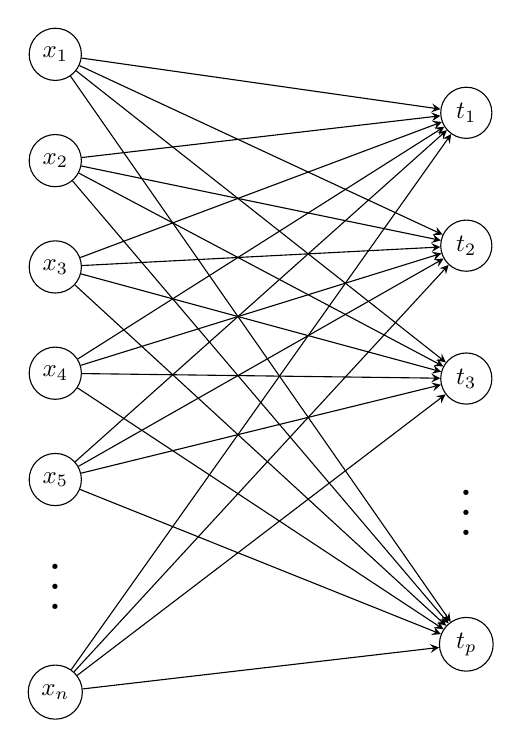
\begin{tikzpicture}[x=2.9cm, y=1.5cm, >=stealth, transform shape, scale=.9]

\foreach \m/\l [count=\y] in {1,...,5}
  \node [every neuron/.try, neuron \m/.try] (input-\m) at (0,3.5-\y) {$x_{\m}$};
  \node [neuron missing/.try] (input-missing) at (0,3.5-6) {};
  \node [every neuron/.try] (input-6) at (0,3.5-7) {$x_n$};

\foreach \h [count=\y] in {1,...,3}
  \node [every neuron/.try] (hidden-\h) at (2,3.2-\y*1.25) {$t_{\h}$};
  \node [neuron missing/.try] (hidden-missing) at (2,3.2-4*1.25) {};
  \node [every neuron/.try] (hidden-4) at (2,3.2-5*1.25) {$t_p$};

\foreach \i in {1,...,6}
  \foreach \j in {1,...,4}
    \draw [->] (input-\i) -- (hidden-\j);

\end{tikzpicture}
\caption{full connection}
\label{fig:full_con_nn}
\end{subfigure}\hfill
\begin{subfigure}[b]{.4\textwidth}
\centering
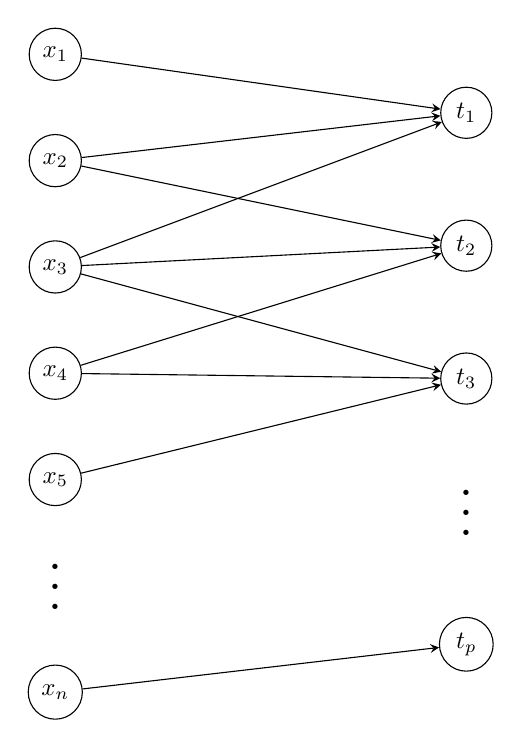
\begin{tikzpicture}[x=2.9cm, y=1.5cm, >=stealth, transform shape, scale=.9]

\foreach \m/\l [count=\y] in {1,...,5}
  \node [every neuron/.try, neuron \m/.try] (input-\m) at (0,3.5-\y) {$x_{\m}$};
  \node [neuron missing/.try] (input-missing) at (0,3.5-6) {};
  \node [every neuron/.try] (input-6) at (0,3.5-7) {$x_n$};

\foreach \h [count=\y] in {1,...,3}
  \node [every neuron/.try] (hidden-\h) at (2,3.2-\y*1.25) {$t_{\h}$};
  \node [neuron missing/.try] (hidden-missing) at (2,3.2-4*1.25) {};
  \node [every neuron/.try] (hidden-4) at (2,3.2-5*1.25) {$t_p$};

\foreach \i in {1,...,3}
    \draw [->] (input-\i) -- (hidden-1);
\foreach \i in {2,...,4}
    \draw [->] (input-\i) -- (hidden-2);
\foreach \i in {3,...,5}
    \draw [->] (input-\i) -- (hidden-3);
\draw [->] (input-6) -- (hidden-4);

\end{tikzpicture}
\caption{local connection}
\label{fig:local_con_nn}
\end{subfigure}
\caption{nn plot example}
\label{fig:nn}
\end{figure}



\bibliographystyle{IEEEtran}
\bibliography{IEEEabrv, references}


% \begin{IEEEbiography}
% [{\includegraphics[width=1in, height=1.25in, clip, keepaspectratio]{bio_images/bio_wenhao.jpg}}]{Hao Wen}
% \end{IEEEbiography}


\end{document}

